\documentclass[compress]{beamer}
\usecolortheme{default}

\usepackage{lmodern, epstopdf, multirow, array, setspace, bbm, tcolorbox, pbox, bm, mathtools, tikz}
\usepackage[T1]{fontenc}

\setbeamertemplate{frametitle}[default][center]
\setbeamertemplate{footline}{\hfill \insertframenumber/\inserttotalframenumber\hspace*{5pt}\vspace{5pt}}
\setbeamertemplate{navigation symbols}{}

\newlength{\wideitemsep}
\setlength{\wideitemsep}{\itemsep}
\addtolength{\wideitemsep}{4pt}
\let\olditem\item
\renewcommand{\item}{\setlength{\itemsep}{\wideitemsep}\olditem}
\setlength{\leftmargini}{12pt}
\setlength{\leftmarginii}{14pt}
\setbeamertemplate{itemize/enumerate subbody begin}{\vspace{6pt}}
\setbeamertemplate{itemize item}[circle]
\setbeamertemplate{enumerate item}[circle]
\setbeamertemplate{enumerate subitem}[default]

\setbeamercolor{alerted text}{fg=blue}
\setbeamersize{text margin left=1.5em,text margin right=1.5em}

\tcbset{
    colback=white,
    colframe=black,
    coltext=black,
    coltitle=blue,
    colbacktitle=white,
    boxrule=1pt,
    titlerule=0pt,
    toptitle=4pt,
    top=2pt
}

\newenvironment{changemargin}[2]{% 
  \begin{list}{}{% 
    \setlength{\topsep}{0pt}% 
    \setlength{\leftmargin}{#1}% 
    \setlength{\rightmargin}{#2}% 
    \setlength{\listparindent}{\parindent}% 
    \setlength{\itemindent}{\parindent}% 
    \setlength{\parsep}{\parskip}% 
  }% 
  \item[]}{\end{list}}
  
\newenvironment{defn}{%
  \begin{tcolorbox}[title={Definition}]%
  }{\end{tcolorbox}}
  
\newenvironment{prop}[1]{%
  \begin{tcolorbox}[title={Proposition #1}]%
  }{\end{tcolorbox}}
  
\newcommand{\cit}[1]{{\footnotesize \textcolor[rgb]{0.5,0,0}{#1}}}

% Font size for code listings (verbatim blocks); reset with \normalsize
\newcommand{\codesize}{\fontsize{7}{8.5}\selectfont}

\newcommand{\slidesetup}[1]{%
  \title{#1}%
  \subtitle{\texorpdfstring{\vspace{0.3\baselineskip}}{} {\small This version: \today}}%
  \author[Mikkel Plagborg-Moller]{ECMA 31150, Spring 2026 \texorpdfstring{\\[0.5ex]}{} University of Chicago \texorpdfstring{\\[0.5ex]}{} Department of Economics \texorpdfstring{\\[4ex]}{} Mikkel Plagborg-Moller}%
  \date{}%
}

% \circleoverlay[options]{text}
% Draws a red circle with a text box nearby on a tikz overlay.
% Options (with defaults):
%   cx=0cm, cy=0cm      - circle center (shift from page center)
%   r=1cm               - circle radius
%   tx=0cm, ty=0cm      - text box offset from circle center
%   text anchor=east    - anchor of text node (east = text left, west = text right)
%   font=\normalsize    - font size for text
\pgfkeys{
  /circleoverlay/.cd,
  cx/.store in=\cocx, cx=0cm,
  cy/.store in=\cocy, cy=0cm,
  r/.store in=\cor, r=1cm,
  tx/.store in=\cotx, tx=0cm,
  ty/.store in=\coty, ty=0cm,
  text anchor/.store in=\cotextanchor, text anchor=east,
  font/.store in=\cofont, font=\normalsize,
}
\newcommand{\circleoverlay}[2][]{%
  \pgfkeys{/circleoverlay/.cd, cx=0cm, cy=0cm, r=1cm, tx=0cm, ty=0cm, text anchor=east, font=\normalsize, #1}%
  \pgfmathsetlengthmacro{\circlediameter}{2*\cor}%
  \node[draw=red, line width=2pt, circle, minimum size=\circlediameter, inner sep=0pt]
    (tmpcirc) at ([xshift=\cocx,yshift=\cocy]current page.center) {};%
  \node[anchor=\cotextanchor, fill=white, draw=red, text=red, inner sep=4pt, align=left, font=\cofont]
    at ([xshift=\cotx,yshift=\coty]tmpcirc.center) {#2};%
}

\DeclareMathOperator*{\argmax}{argmax}
\DeclareMathOperator*{\argmin}{argmin}
\DeclareMathOperator{\diag}{diag}
\DeclareMathOperator{\var}{Var}
\DeclareMathOperator{\cov}{Cov}
\DeclareMathOperator{\corr}{Corr}
\DeclareMathOperator{\lrv}{LRV}


\slidesetup{Inference with weakly dependent data I}

\begin{document}
\frame{
\maketitle
}

\frame{
\frametitle{Plan for this slide deck}
\begin{enumerate}
\item Standard errors for general time series regression
\item CLT for weakly dependent data
\item Heteroskedasticity and autocorrelation consistent (HAC) estimator, Newey-West SE
\item Application: testing forecast rationality
\end{enumerate}
}

\frame{
\frametitle{Time series regression}
\begin{itemize}
\item Given jointly covariance stationary time series $\lbrace y_t,x_t \rbrace$, consider an OLS regression of $y_t$ on $x_t$:
\[y_t = \hat{\beta}_0 + \hat{\beta}_1 x_t + \hat{v}_t.\]
\item How should we compute standard errors for the coefficients?
\item In our discussion of AR models, we have seen that if
\[y_t = \beta_0 + \beta_1 x_t + v_t,\]
and $\lbrace v_t \rbrace$ is a martingale difference sequence, then we can use the usual SE formula for i.i.d.\ regressions.
\item But in many cases, we may expect $v_t$ to be serially correlated (and therefore certainly not a MDS).
\end{itemize}
}

\frame{
\frametitle{The Phillips curve: $\corr(\text{inflation},\text{unemployment})<0$}
\begin{figure}
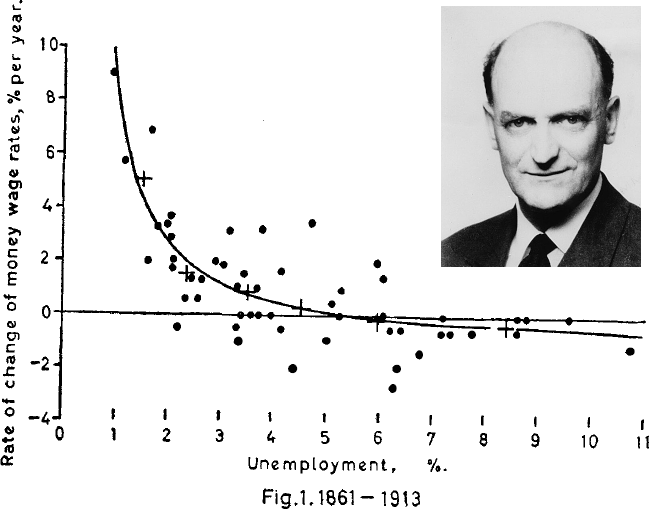
\includegraphics[width=0.75\linewidth]{fig/phillips_1958_fig1.png} \\[1ex]
\hfill \footnotesize Note: UK data. Source: Phillips (1958)
\end{figure}
}

\frame{
\begin{figure}
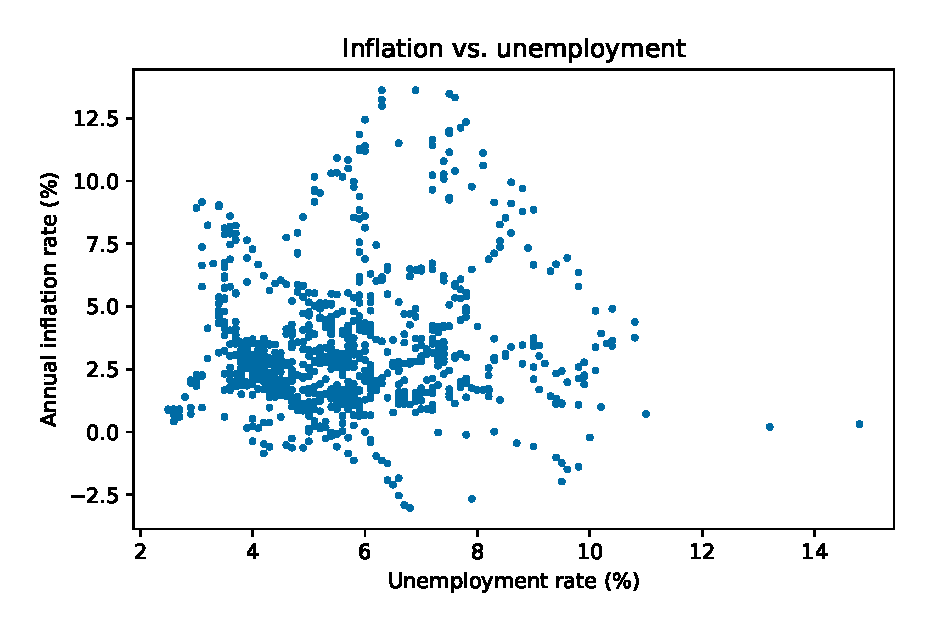
\includegraphics[width=\linewidth]{fig/scatter_infl_unemp.eps} \\
U.S. data 1948--2026 \\
Inflation: log change in CPI relative to 12 months ago
\end{figure}
}

\begin{frame}[fragile]
\scriptsize
\begin{verbatim}
                            OLS Regression Results                            
==============================================================================
Dep. Variable:              inflation   R-squared:                       0.006
Model:                            OLS   Adj. R-squared:                  0.005
Method:                 Least Squares   F-statistic:                     4.746
Date:                Mon, 13 Apr 2026   Prob (F-statistic):             0.0296
Time:                        20:22:43   Log-Likelihood:                -2227.8
No. Observations:                 926   AIC:                             4460.
Df Residuals:                     924   BIC:                             4469.
Df Model:                           1                                         
Covariance Type:                  HC1                                         
==============================================================================
                 coef    std err          z      P>|z|      [0.025      0.975]
------------------------------------------------------------------------------
const          2.6917      0.295      9.119      0.000       2.113       3.270
UNRATE         0.1190      0.055      2.178      0.029       0.012       0.226
==============================================================================
Omnibus:                      195.796   Durbin-Watson:                   0.024
Prob(Omnibus):                  0.000   Jarque-Bera (JB):              379.007
Skew:                           1.228   Prob(JB):                     5.01e-83
Kurtosis:                       4.947   Cond. No.                         21.3
==============================================================================

Notes:
[1] Standard Errors are heteroscedasticity robust (HC1)
\end{verbatim}
\end{frame}

\frame{
\begin{figure}
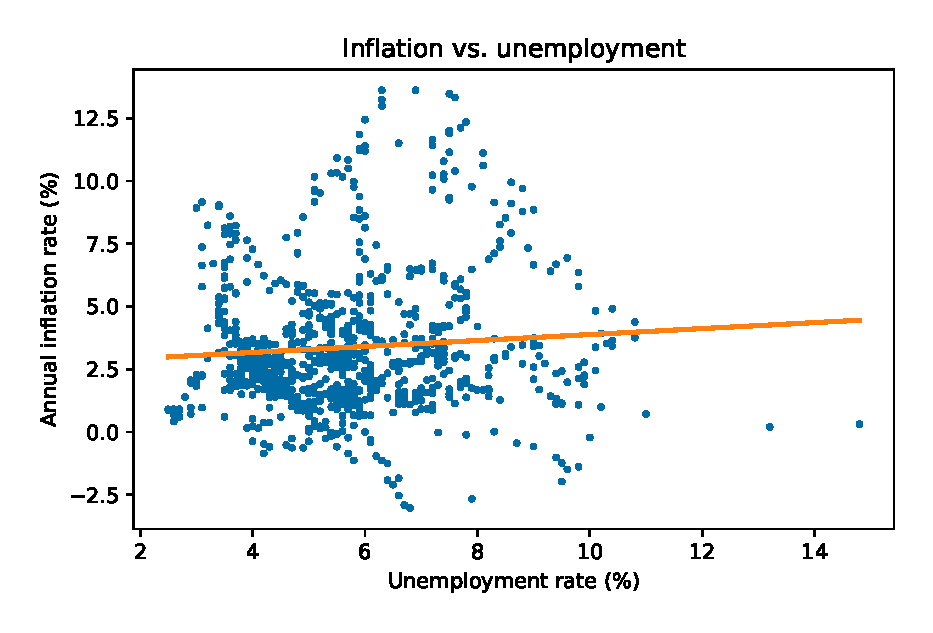
\includegraphics[width=\linewidth]{fig/scatter_infl_unemp_ols.eps}
\end{figure}
}

\frame{
\begin{figure}
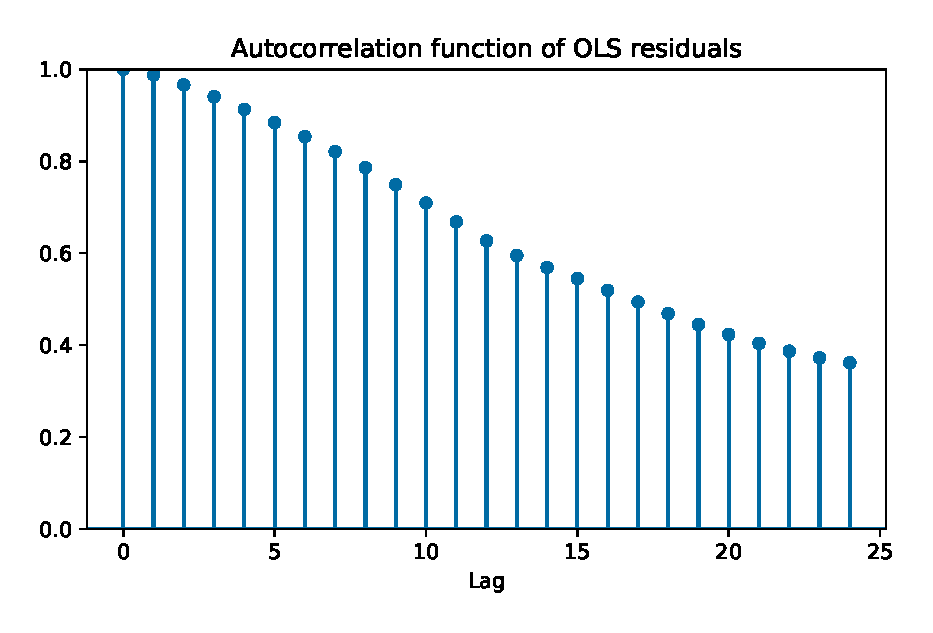
\includegraphics[width=\linewidth]{fig/acf_resid.eps} \\
$\lbrace \hat{v}_t \rbrace$ definitely doesn't look like white noise!
\end{figure}
}

\frame{
\frametitle{Distribution of OLS estimator}
\begin{itemize}
\item Drop the intercept for now and assume the linear model
\[y_t = \beta x_t + v_t,\quad E[x_tv_t]=0.\]
\vspace{-1.3\baselineskip}
\begin{itemize}
\item Not really an assumption. Can always define the \textbf{best linear prediction} coefficient
\[\beta \equiv \argmin_b E\left[(y_t-x_t b)^2\right],\quad \text{and} \quad v_t \equiv y_t-\beta x_t.\]
Then the FOC implies $E[x_tv_t]=0$.
\end{itemize}
\item OLS estimator of $\beta$:
\[\hat{\beta} \equiv \frac{\sum_{t=1}^T y_tx_t}{\sum_{t=1}^T x_t^2} = \beta + \frac{\sum_{t=1}^T v_tx_t}{\sum_{t=1}^T x_t^2}\]
\[\Longrightarrow \sqrt{T}(\hat{\beta}-\beta) =  \frac{\frac{1}{\sqrt{T}}\sum_{t=1}^T v_tx_t}{\frac{1}{T}\sum_{t=1}^T x_t^2}.\]
\end{itemize}
}

\frame{
\frametitle{Distribution of OLS estimator (cont.)}
\begin{equation} \label{eqn:ols}
\sqrt{T}(\hat{\beta}-\beta) =  \frac{\frac{1}{\sqrt{T}}\sum_{t=1}^T v_tx_t}{\frac{1}{T}\sum_{t=1}^T x_t^2} \tag{$\dagger$}
\end{equation}
\begin{itemize}
\item It turns out that the denominator in (\ref{eqn:ols}) satisfies the law of large numbers (LLN) provided that $\lbrace x_t \rbrace$ is stationary and $\lim_{\ell\to\infty}\cov(x_t^2,x_{t-\ell}^2) = 0$:
\[\frac{1}{T}\sum_{t=1}^T x_t^2 \overset{p}{\to} E[x_t^2]\quad \text{as}\quad T\to\infty.\]
\item The numerator in (\ref{eqn:ols}) is a scaled sample average of terms with mean zero (by assumption). Does it satisfy a central limit theorem (CLT)?
\end{itemize}
}

\frame{
\frametitle{CLT with dependent data}
\begin{itemize}
\item A simple example shows that the CLT can indeed hold (in modified form) for dependent data.
\item Consider the MA(1) process
\[y_t = u_t + \theta u_{t-1},\quad u_t \overset{iid}{\sim} (0,\sigma^2).\]
\item Then
{\small
\begin{align*}
\frac{1}{\sqrt{T}}\sum_{t=1}^T y_t &= \frac{1}{\sqrt{T}}\Big( u_1 + \theta u_0 + u_2 + \theta u_1 + u_3 + \theta u_2 + \dots + u_T + \theta u_{T-1}\Big) \\
&= (1+\theta)\underbrace{\frac{1}{\sqrt{T}}\sum_{t=1}^T u_t}_{\overset{d}{\to} N(0,\sigma^2)} + \underbrace{\frac{1}{\sqrt{T}}\theta(u_0 - u_T)}_{\overset{p}{\to} 0} \overset{d}{\to} \boxed{N\Big(0, (1+\theta)^2\sigma^2\Big)},
\end{align*}
}
using the usual CLT for i.i.d.\ variables (the $u_t$'s) and Slutsky's thm.
\end{itemize}
}

\frame{
\frametitle{CLT with dependent data (cont.)}
\[y_t = u_t + \theta u_{t-1},\quad u_t \overset{iid}{\sim} (0,\sigma^2)\]
\begin{itemize}
\item In this example, the asymptotic variance of the scaled sample average is
\[(1+\theta)^2\sigma^2,\]
even though
\[\var(y_t) = (1+\theta^2)\sigma^2.\]
(Recall the formula for the variance of an MA process.)
\item So something is different when applying the CLT to dependent processes, relative to the i.i.d.\ case: we still get asymptotic normality, but the variance is different.
\end{itemize}
}

\frame{
\frametitle{Variance of sample mean}
\begin{itemize}
\item Let's derive the variance of the scaled sample mean of a general covariance stationary process $\lbrace y_t \rbrace$ with autocovariances $\gamma(\ell)$.
\item Then
\begin{align*}
&\var\left(\frac{1}{\sqrt{T}}\sum_{t=1}^T y_t\right) = \frac{1}{T} \sum_{t=1}^T \sum_{s=1}^T \cov(y_t,y_s) \\
&= \frac{1}{T} \sum_{t=1}^T \sum_{s=1}^T \gamma(t-s) = \gamma(0) + 2\sum_{\ell=1}^{T-1} \frac{T-\ell}{T} \gamma(\ell).
\end{align*}
\vspace{-\baselineskip}
\begin{itemize}
\item \alert{Exercise:} Make sure you understand each step.
\end{itemize}
\end{itemize}
}

\frame{
\frametitle{Variance of sample mean (cont.)}
\[\var\left(\frac{1}{\sqrt{T}}\sum_{t=1}^T y_t\right) = \gamma(0) + 2\sum_{\ell=1}^{T-1} \frac{T-\ell}{T} \gamma(\ell)\]
\begin{itemize}
\item Assume that the process $\lbrace y_t \rbrace$ is \textbf{weakly dependent} in the sense that
\[\sum_{\ell=1}^\infty |\gamma(\ell)| < \infty.\]
\vspace{-\baselineskip}
\begin{itemize}
\item Requires $\gamma(\ell) \to 0$ sufficiently fast as $\ell \to \infty$.
\end{itemize}
\item Then the ``dominated convergence theorem'' implies
\[\boxed{\lim_{T\to\infty} \var\left(\frac{1}{\sqrt{T}}\sum_{t=1}^T y_t\right) = \gamma(0) + 2\sum_{\ell=1}^\infty \gamma(\ell)}.\]
\end{itemize}
}

\frame{
\frametitle{Long-run variance}
\[\lim_{T\to\infty}\var\left(\frac{1}{\sqrt{T}}\sum_{t=1}^T y_t\right) = \gamma(0) + 2\sum_{\ell=1}^\infty \gamma(\ell) \equiv \lrv(y_t)\]
\begin{itemize}
\item LRV: \textbf{long-run variance}.
\item If the process is white noise, then $\lrv(y_t) = \gamma(0) = \var(y_t)$. But otherwise, we generally have $\lrv(y_t) \neq \var(y_t)$.
\item \alert{Exercise:} show that for a cov.\ stationary AR(1) process,
\[\lrv(y_t) = \frac{\sigma^2}{(1-\rho)^2} \neq \frac{\sigma^2}{1-\rho^2} = \var(y_t).\]
\end{itemize}
}

\frame{
\frametitle{CLT with dependent data: result}
\begin{itemize}
\item \alert{Result:} if the process $\lbrace y_t \rbrace$ is stationary, has mean zero, is weakly dependent, and satisfies some other regularity conditions, then
\[\frac{1}{\sqrt{T}}\sum_{t=1}^T y_t \overset{d}{\to} N\Big(0, \lrv(y_t) \Big).\]
\vspace{-\baselineskip}
\begin{itemize}
\item Formal results: Hayashi (2000) textbook, chapter 6.5.
\end{itemize}
\item If the process is positively serially correlated, so that $\gamma(\ell) \geq 0$ for $\ell \geq 1$, then $\lrv(y_t) \geq \var(y_t)$.
\item So compared with the case of i.i.d.\ data, the sample average of a positively serially correlated time series has higher variance.
\begin{itemize}
\item It's effectively as if the sample size is smaller: we observe fewer (nearly) independent observations.
\end{itemize}
\end{itemize}
}

\frame{
\begin{figure}
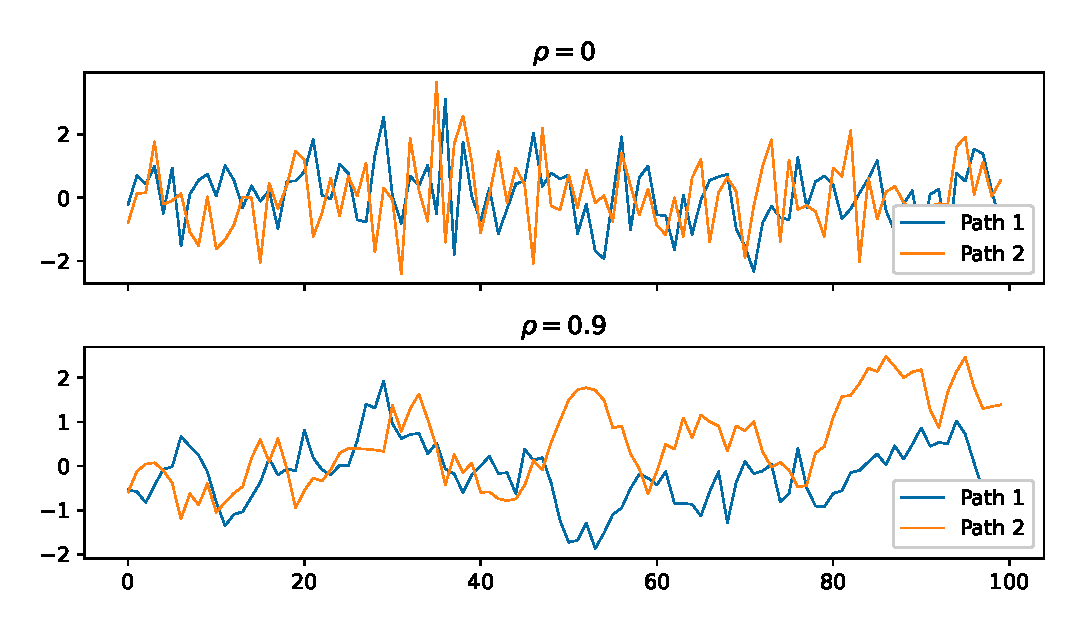
\includegraphics[width=0.9\linewidth]{fig/ar1_sim.eps}
\end{figure}
\begin{itemize}
\item The plot shows two AR(1) processes with different persistence $\rho$, each normalized to have variance = 1.
\item The white noise process (top) averages out the noise/shocks much faster than the persistent process (bottom).
\end{itemize}
}

\frame{
\frametitle{Long-run variance: linear filter}
\begin{itemize}
\item \alert{Result:} suppose $y_t = b(L) x_t$ for some (absolutely summable) linear filter $b(L) \equiv \sum_{\ell=-\infty}^\infty b_\ell L^\ell$. Then
\[\lrv(y_t) = [b(1)]^2 \times \lrv(x_t).\]
\vspace{-1.5\baselineskip}
\begin{itemize}
\item Recall: $b(1) \equiv \sum_{\ell=-\infty}^\infty b_\ell$.
\end{itemize}
\item \alert{Exercise:} show that the MA(1) process $y_t = u_t + \theta u_{t-1}$, with $u_t \sim \mathit{WN}(\sigma^2)$, has $\lrv(y_t) = (1+\theta)^2\sigma^2$.
\begin{itemize}
\item Consistent with our earlier expression for the asymptotic variance of the sample average of this process.
\end{itemize}
\end{itemize}
}

\frame{
\frametitle{Distribution of OLS estimator: conclusion}
\begin{itemize}
\item Back to the OLS estimator:
\[\sqrt{T}(\hat{\beta}-\beta) =  \frac{\frac{1}{\sqrt{T}}\sum_{t=1}^T v_tx_t}{\frac{1}{T}\sum_{t=1}^T x_t^2}.\]
\item We have seen that, under some weak conditions,
\[\frac{1}{T}\sum_{t=1}^T x_t^2 \overset{p}{\to} E[x_t^2],\quad \text{and}\quad  \frac{1}{\sqrt{T}}\sum_{t=1}^T v_tx_t \overset{d}{\to} N\Big(0, \lrv(v_tx_t)\Big).\]
\item Hence, by Slutsky's theorem,
\[\boxed{\sqrt{T}(\hat{\beta}-\beta) \overset{d}{\to} N\left(0, \frac{\lrv(v_tx_t)}{\left(E[x_t^2]\right)^2} \right)}.\]
\end{itemize}
}

\frame{
\frametitle{Standard errors for time series regression}
\begin{itemize}
\item Written a bit more loosely, when $T$ is large,
\[\hat{\beta} \overset{approx}{\sim} N\left(\beta, \frac{1}{T} \times \frac{\lrv(v_tx_t)}{\left(E[x_t^2]\right)^2} \right).\]
\item For this to be useful for inference, we need to estimate the variance.
\item Suppose we had a consistent estimator $\widehat{\lrv}$ of $\lrv(v_tx_t)$. Then we could use the standard errors
\[\mathit{SE}(\hat{\beta}) \equiv \sqrt{\frac{1}{T} \times \frac{\widehat{\lrv}}{\left(\frac{1}{T}\sum_{t=1}^T x_t^2\right)^2}}.\]
\item How to consistently estimate the LRV?
\end{itemize}
}

\frame{
\frametitle{Long-run variance: estimation}
\[\lrv(y_t) \equiv \sum_{\ell=-\infty}^\infty \gamma(\ell) = \gamma(0) + 2\sum_{\ell=1}^\infty \gamma(\ell)\]
\begin{itemize}
\item Most natural estimator:
\[\widetilde{LRV} \equiv \hat{\gamma}(0) + 2\sum_{\ell=1}^{T-1} \hat{\gamma}(\ell),\]
using the sample autocovariances
\[\hat{\gamma}(\ell) \equiv \frac{1}{T}\sum_{t=\ell+1}^{T} (y_t-\bar{y})(y_{t-\ell}-\bar{y}),\quad \ell=0,1,\dots,T-1.\]
\item But this estimator turns out to be \emph{inconsistent}! (In fact, it equals 0.)
\item Intuitively, $\hat{\gamma}(\ell)$ is a poor estimator of $\gamma(\ell)$ for $\ell \approx T$.
\end{itemize}
}

\frame{
\frametitle{Long-run variance: estimation (cont.)}
\begin{itemize}
\item Consider instead the weighted estimator
\[\widehat{LRV} \equiv \hat{\gamma}(0) + 2\sum_{\ell=1}^{B} K\left(\frac{\ell}{B}\right) \hat{\gamma}(\ell),\]
where $K \colon [0,1] \to [-1,1]$ is a function called the \textbf{kernel}, and $B$ is an integer called the \textbf{bandwidth}. We require $K(0)=1$.
\begin{itemize}
\item $\widehat{LRV}$ sums over a smaller number $B$ of autocovariances. Can use the kernel to down-weight the noisy estimates at longer lags $\ell \approx B$.
\end{itemize}
\item \alert{Result:} if $B=B(T)$ is a function of $T$ such that $B \to \infty$ and $B/T \to 0$ (and some other regularity conditions hold), then $\widehat{LRV}$ is consistent.
\item We call $\widehat{LRV}$ a \textbf{heteroskedasticity and autocorrelation consistent} (HAC) estimator.
\end{itemize}
}

\begin{frame}[fragile]
\frametitle{Long-run variance: Newey-West estimator}
\begin{itemize}
\item By far the most popular HAC estimator is the \textbf{Newey-West} estimator. It sets $K(x) = 1-x$ (the \textbf{Bartlett kernel}):
\[\widehat{LRV}_\text{NW} \equiv \hat{\gamma}(0) + 2\sum_{\ell=1}^{B-1} \left(1-\frac{\ell}{B}\right) \hat{\gamma}(\ell),\]
\item Rule of thumb bandwidth from Stock \& Watson textbook: $B = 0.75 \times T^{1/3}$ (rounded up).
\item To compute OLS standard errors, we need $\lrv(x_tv_t)$. Estimate this by applying the Newey-West formula to the sample autocovariances of the series $\lbrace x_t\hat{v}_t \rbrace$, where $\hat{v}_t$ are the OLS residuals.
\end{itemize}
\end{frame}

\begin{frame}[fragile]
\begin{verbatim}
# OLS regression with Newey-West SE
T_nw = model.nobs
nw_bw = int(np.ceil(0.75 * T_nw**(1/3)))
model_nw = sm.OLS(df['inflation'], X).fit(cov_type='HAC',
    cov_kwds={'maxlags': nw_bw-1})
print(model_nw.summary())
\end{verbatim}
\medskip
Note: \texttt{maxlags} $= B-1$
\end{frame}

\begin{frame}[fragile]
\scriptsize
\begin{verbatim}
                            OLS Regression Results                            
==============================================================================
Dep. Variable:              inflation   R-squared:                       0.006
Model:                            OLS   Adj. R-squared:                  0.005
Method:                 Least Squares   F-statistic:                    0.7345
Date:                Mon, 13 Apr 2026   Prob (F-statistic):              0.392
Time:                        20:22:43   Log-Likelihood:                -2227.8
No. Observations:                 926   AIC:                             4460.
Df Residuals:                     924   BIC:                             4469.
Df Model:                           1                                         
Covariance Type:                  HAC                                         
==============================================================================
                 coef    std err          z      P>|z|      [0.025      0.975]
------------------------------------------------------------------------------
const          2.6917      0.743      3.622      0.000       1.235       4.148
UNRATE         0.1190      0.139      0.857      0.391      -0.153       0.391
==============================================================================
Omnibus:                      195.796   Durbin-Watson:                   0.024
Prob(Omnibus):                  0.000   Jarque-Bera (JB):              379.007
Skew:                           1.228   Prob(JB):                     5.01e-83
Kurtosis:                       4.947   Cond. No.                         21.3
==============================================================================

Notes:
[1] Standard Errors are heteroscedasticity and autocorrelation robust (HAC)
using 7 lags and without small sample correction
\end{verbatim}
\uncover<2>{%
\begin{tikzpicture}[overlay, remember picture]
  \circleoverlay[cx=-1.4cm, cy=-0.6cm, r=0.43cm,
                 tx=0.5cm, ty=-0.8cm, text anchor=west]{2.5 $\times$ larger than \\ non-HAC SE!}
\end{tikzpicture}%
}
\end{frame}

\frame{
\frametitle{Extensions}
\begin{itemize}
\item Straight-forward generalization to multivariate regression:
\[y_t = \hat{\beta}_0 + \hat{\beta}_1 x_{1t} + \dots + \hat{\beta}_k x_{kt} + \hat{v}_t.\]
\vspace{-1.5\baselineskip}
\begin{itemize}
\item CLT and HAC estimator can be extended to vector processes.
\item F-test for time series data.
\item Most statistics software can do all this for you.
\end{itemize}
\item HAC estimation typically does not work well in small samples when the data is highly persistent. Can ameliorate this by using a larger bandwidth $B$ and adjusting the critical value of our tests/CIs.
\begin{itemize}
\item Review of state of the art: Lazarus, Lewis, Stock \& Watson (2018).
\end{itemize}
\end{itemize}
}

\begin{frame}[fragile]
\scriptsize
\begin{verbatim}
                            OLS Regression Results                            
==============================================================================
Dep. Variable:              inflation   R-squared:                       0.235
Model:                            OLS   Adj. R-squared:                  0.233
Method:                 Least Squares   F-statistic:                     17.19
Date:                Mon, 13 Apr 2026   Prob (F-statistic):           4.70e-08
Time:                        20:22:43   Log-Likelihood:                -2106.7
No. Observations:                 926   AIC:                             4219.
Df Residuals:                     923   BIC:                             4234.
Df Model:                           2                                         
Covariance Type:                  HAC                                         
==============================================================================
                 coef    std err          z      P>|z|      [0.025      0.975]
------------------------------------------------------------------------------
const          1.9934      0.737      2.705      0.007       0.549       3.438
UNRATE         0.2086      0.136      1.536      0.124      -0.057       0.475
oil_change     0.0454      0.008      5.822      0.000       0.030       0.061
==============================================================================
Omnibus:                      104.306   Durbin-Watson:                   0.047
Prob(Omnibus):                  0.000   Jarque-Bera (JB):              146.152
Skew:                           0.837   Prob(JB):                     1.83e-32
Kurtosis:                       3.992   Cond. No.                         103.
==============================================================================

Notes:
[1] Standard Errors are heteroscedasticity and autocorrelation robust (HAC)
using 7 lags and without small sample correction
\end{verbatim}
\medskip
\normalsize
Extra covariate: 12-month log change in oil price (WTI crude)
\end{frame}

\frame{
\frametitle{Another application: testing forecast rationality}
\begin{itemize}
\item Mankiw, Reis \& Wolfers (2003) test (among other things) whether forecasts of inflation $\pi_t$ are rational.
\item Forecast sources:
\begin{itemize}
\item Michigan survey of households
\item Livingston and SPF surveys of professional forecasters
\end{itemize}
\item Regress 12-month-ahead forecast errors $\pi_t - \pi_{t|t-12}$ on various time series to test if the errors can be systematically predicted.
\item The multi-step forecast errors must be serially correlated (even if forecasts were rational), since they depend on all shocks that hit the economy between time $t-12$ and $t$. \\
\smallskip
$\Longrightarrow$ Need Newey-West SE.
\end{itemize}
}

\frame{
\begin{figure}
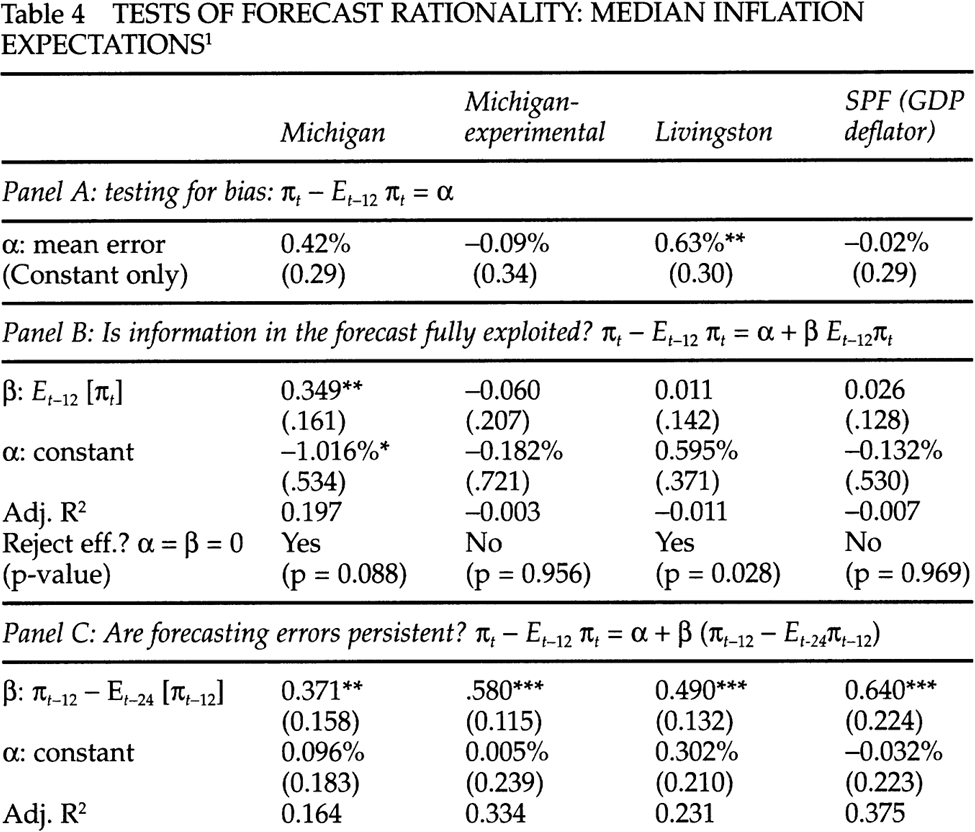
\includegraphics[width=0.8\linewidth]{fig/mrw_tab4a.png} \\
\smallskip
\footnotesize Source: Mankiw, Reis \& Wolfers (2003)
\end{figure}
}

\frame{
\begin{figure}
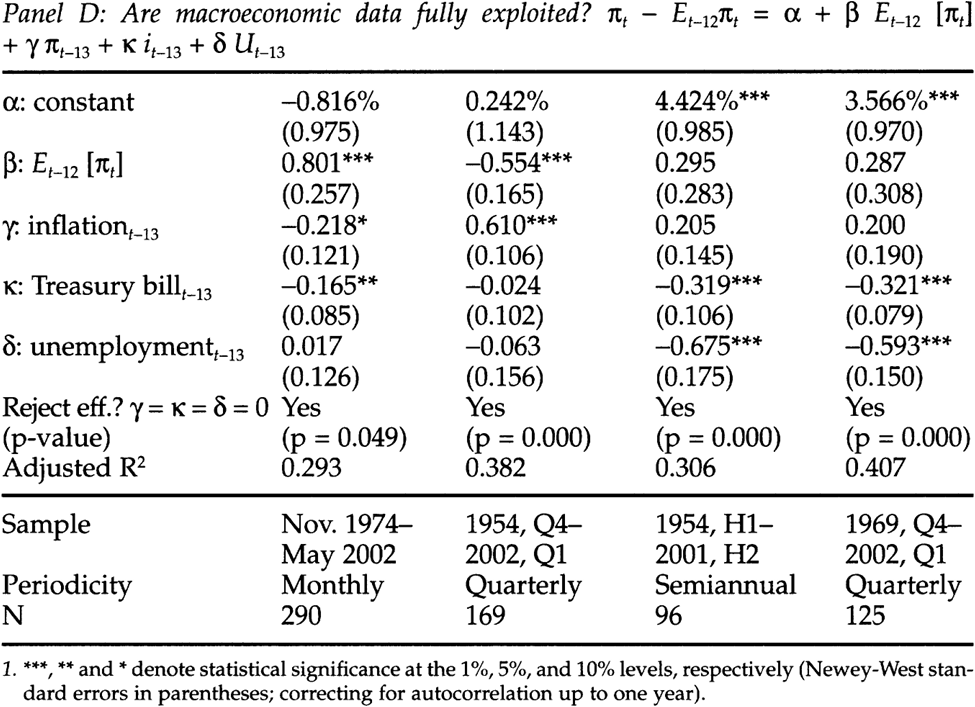
\includegraphics[width=0.8\linewidth]{fig/mrw_tab4b.png} \\
\smallskip
\footnotesize Source: Mankiw, Reis \& Wolfers (2003)
\end{figure}
}

\frame{
\frametitle{Data frequency and efficiency}
\begin{itemize}
\item Suppose we've run a regression on quarterly data. Then we realize that the series are also available at monthly frequency over the same time span.
\item Using the monthly data, our sample size $T$ triples. Naively, we might expect our OLS SE to decrease by a factor of $\sqrt{3} \approx 1.73$.
\item But in most cases in practice, the monthly data will be much more \emph{persistent} than the quarterly data: the relevant LRV is large.
\item Hence, our OLS SE usually do not decrease that much when switching from quarterly to monthly, despite the larger $T$.
\item Of course, monthly data is still useful for analyzing high-frequency dynamics.
\end{itemize}
}

\frame{
\frametitle{What did we learn?}
\begin{itemize}
\item LLN + CLT for dependent data
\item Asymptotic distribution of OLS estimator
\item Long-run variance
\begin{itemize}
\item $>\var$ for positively serially correlated series
\item Formula for linear filters
\item HAC estimation, Newey-West
\end{itemize}
\item SE for time series regression
\end{itemize}
}

\frame{
\frametitle{Looking ahead}
\begin{itemize}
\item Instrumental variables regression with time series data
\item How can we identify whether economic agents are forward-looking or backward-looking?
\begin{itemize}
\item New Keynesian Phillips curve
\item Consumption Euler equation
\end{itemize}
\end{itemize}
}

\end{document}
